\documentclass[a4paper, 12pt]{article}

\RequirePackage[l2tabu, orthodox]{nag}

\usepackage{minted}
\usepackage{graphicx}
\usepackage{amsmath}
\usepackage{fontspec}
\usepackage{unicode-math}
\usepackage{tikz}
\usepackage{adjustbox}
\usepackage{hyperref}
\usepackage{booktabs}
\usepackage{shapepar}

\usepackage[english]{babel}
\usepackage{blindtext}

\usepackage[
  type={CC},
  modifier={by-sa},
  version={4.0}
]{doclicense}

\hypersetup{
  colorlinks=true,
  linkcolor=blue,
  filecolor=magenta,
  urlcolor=cyan
}

\usetikzlibrary{lindenmayersystems}

\setmainfont[Path = fonts/,
  UprightFont = *-Regular,
  BoldFont = *-Bold,
  ItalicFont = *-Italic,
  BoldItalicFont = *-BoldItalic
]{TexGyrePagella}

\setmonofont[Path = fonts/,
  UprightFont = *-Regular,
  BoldFont = *-Bold,
  ItalicFont = *-Italic,
  BoldItalicFont = *-BoldItalic
]{RobotoMono}

\setmathfont[
  Path = fonts/
]{TexGyrePagella-Math}

\newcommand{\pipar}[1]{\shapepar{\pishape}#1\par}
\newcommand{\pishape}{%
  {25.0839}%
  {0.0838926}b{14.3456}\\%
  {0.0838926}t{14.3456}{33.3054}\\%
  {0.503356}t{11.5772}{37.6678}\\%
  {1.25839}t{9.98322}{39.6812}\\%
  {2.09732}t{8.52614}{41.5578}\\%
  {2.85235}t{7.21477}{42.8691}\\%
  {3.27181}t{6.7953}{43.2886}\\%
  {4.11074}t{5.95638}{43.7081}\\%
  {5.28524}t{4.78188}{43.7081}\\%
  {5.62081}t{4.44631}{15.1007}st{19.547}{12.6678}st{32.2148}{15.0168}\\%
  {5.62081}t{4.44631}{7.9698}t{19.547}{2.34899}t{32.2148}{2.34899}\\%
  {6.04027}t{4.18011}{6.22257}t{19.4227}{2.37488}t{32.1424}{2.37047}\\%
  {6.87919}t{3.64772}{5.16101}t{19.1741}{2.42667}t{31.9978}{2.41343}\\%
  {7.63423}t{3.16856}{4.04621}t{18.9504}{2.47328}t{31.8676}{2.45208}\\%
  {8.05369}t{2.90236}{3.80463}t{18.8261}{2.49917}t{31.7953}{2.47356}\\%
  {8.38926}t{2.6894}{3.61137}t{18.7267}{2.51989}t{31.7245}{2.50373}\\%
  {9.22819}t{2.15701}{3.12823}t{18.4781}{2.57167}t{31.5474}{2.57045}\\%
  {9.98322}t{1.67785}{2.96021}t{18.2544}{2.61828}t{31.388}{2.6305}\\%
  {11.5772}t{0.415968}{2.85584}t{17.7821}{2.71667}t{31.0515}{2.75727}\\%
  {11.9966}t{0.0838926}{2.91826}t{17.6578}{2.74256}t{30.9629}{2.79063}\\%
  {12.4161}t{0.0838926}{2.64861}t{17.5336}{2.76846}t{30.8743}{2.82399}\\%
  {12.7517}t{0.0838926}{2.43289}t{17.4088}{2.81003}t{30.8035}{2.85068}\\%
  {13.1711}t{0.0838926}{2.22315}t{17.2529}{2.862}t{30.715}{2.88404}\\%
  {13.5906}t{0.0838926}{2.01342}t{17.097}{2.91397}t{30.6264}{2.9174}\\%
  {14.0101}t{0.0838926}{0.838926}t{16.9411}{2.96594}t{30.5378}{2.95076}\\%
  {14.0101}e{0.922819}t{16.9411}{2.96594}t{30.5378}{2.95076}\\%
  {14.7651}t{16.6605}{3.05948}t{30.3785}{3.01081}\\%
  {15.604}t{16.3487}{3.16342}t{30.2013}{3.18792}\\%
  {16.7785}t{15.9121}{3.30893}t{30.0039}{3.3854}\\%
  {21.896}t{14.0101}{3.94295}t{29.1434}{4.24586}\\%
  {25.0839}t{12.7724}{4.3305}t{28.6074}{4.78188}\\%
  {25.8389}t{12.4793}{4.42229}t{28.6074}{4.78188}\\%
  {29.0268}t{11.2416}{4.80984}t{28.6074}{5.39494}\\%
  {29.4463}t{11.0415}{4.8981}t{28.6074}{5.47561}\\%
  {30.2013}t{10.6813}{5.04094}t{28.6074}{5.62081}\\%
  {30.6208}t{10.4812}{5.12029}t{28.6074}{5.72383}\\%
  {34.9832}t{8.40004}{5.9456}t{28.9901}{6.41263}\\%
  {35.4027}t{8.19993}{6.00914}t{29.0268}{6.58557}\\%
  {37.3322}t{7.27942}{6.30143}t{29.5346}{7.04256}\\%
  {38.1711}t{6.87919}{6.42852}t{29.7554}{6.64702}\\%
  {38.5906}t{6.87919}{6.29195}t{29.8658}{6.44925}\\%
  {39.3456}t{7.09492}{5.59084}t{30.1612}{5.9965}\\%
  {39.7651}t{7.21477}{5.20134}t{30.3254}{5.4129}\\%
  {40.5201}t{7.63423}{4.24257}t{30.6208}{4.36242}\\%
  {40.9396}t{8.01175}{3.56544}t{31.2081}{2.60067}\\%
  {41.3591}t{8.38926}{2.43289}t{31.7953}{0.838926}\\%
  {41.3591}e{10.8221}e{32.6342}%
}

\title{\LaTeX}
\author{José Ignacio Escribano}

% Metadata
\hypersetup{
    pdfauthor={José Ignacio Escribano},
    pdftitle={LaTeX},
    pdfkeywords={LaTeX},
}

\begin{document}

  \maketitle

  \doclicenseThis

  \tableofcontents

  \newpage

  \section{\LaTeX}

  \LaTeX{} is a document preparation system for
  the \TeX{} typesetting program. It offers
  programmable desktop publishing features and
  extensive facilities for automating most
  aspects of typesetting and desktop publishing,
  including numbering and cross-referencing,
  tables and figures, page layout,
  bibliographies, and much more. \LaTeX{} was
  originally written in 1984 by Leslie Lamport
  and has become the  dominant method for using
  \TeX; few people write in plain \TeX{} anymore.
  The current version is \LaTeXe.

  \begin{align}
    E_0 &= mc^2 \\
    E &= \frac{mc^2}{\sqrt{1-\frac{v^2}{c^2}}}
  \end{align}

  The most famous book to learn \TeX{} and \LaTeX{}
  are~\cite{texbook} and~\cite{latex}, respectively.

  \begin{figure}[htbp!]
    \centering
    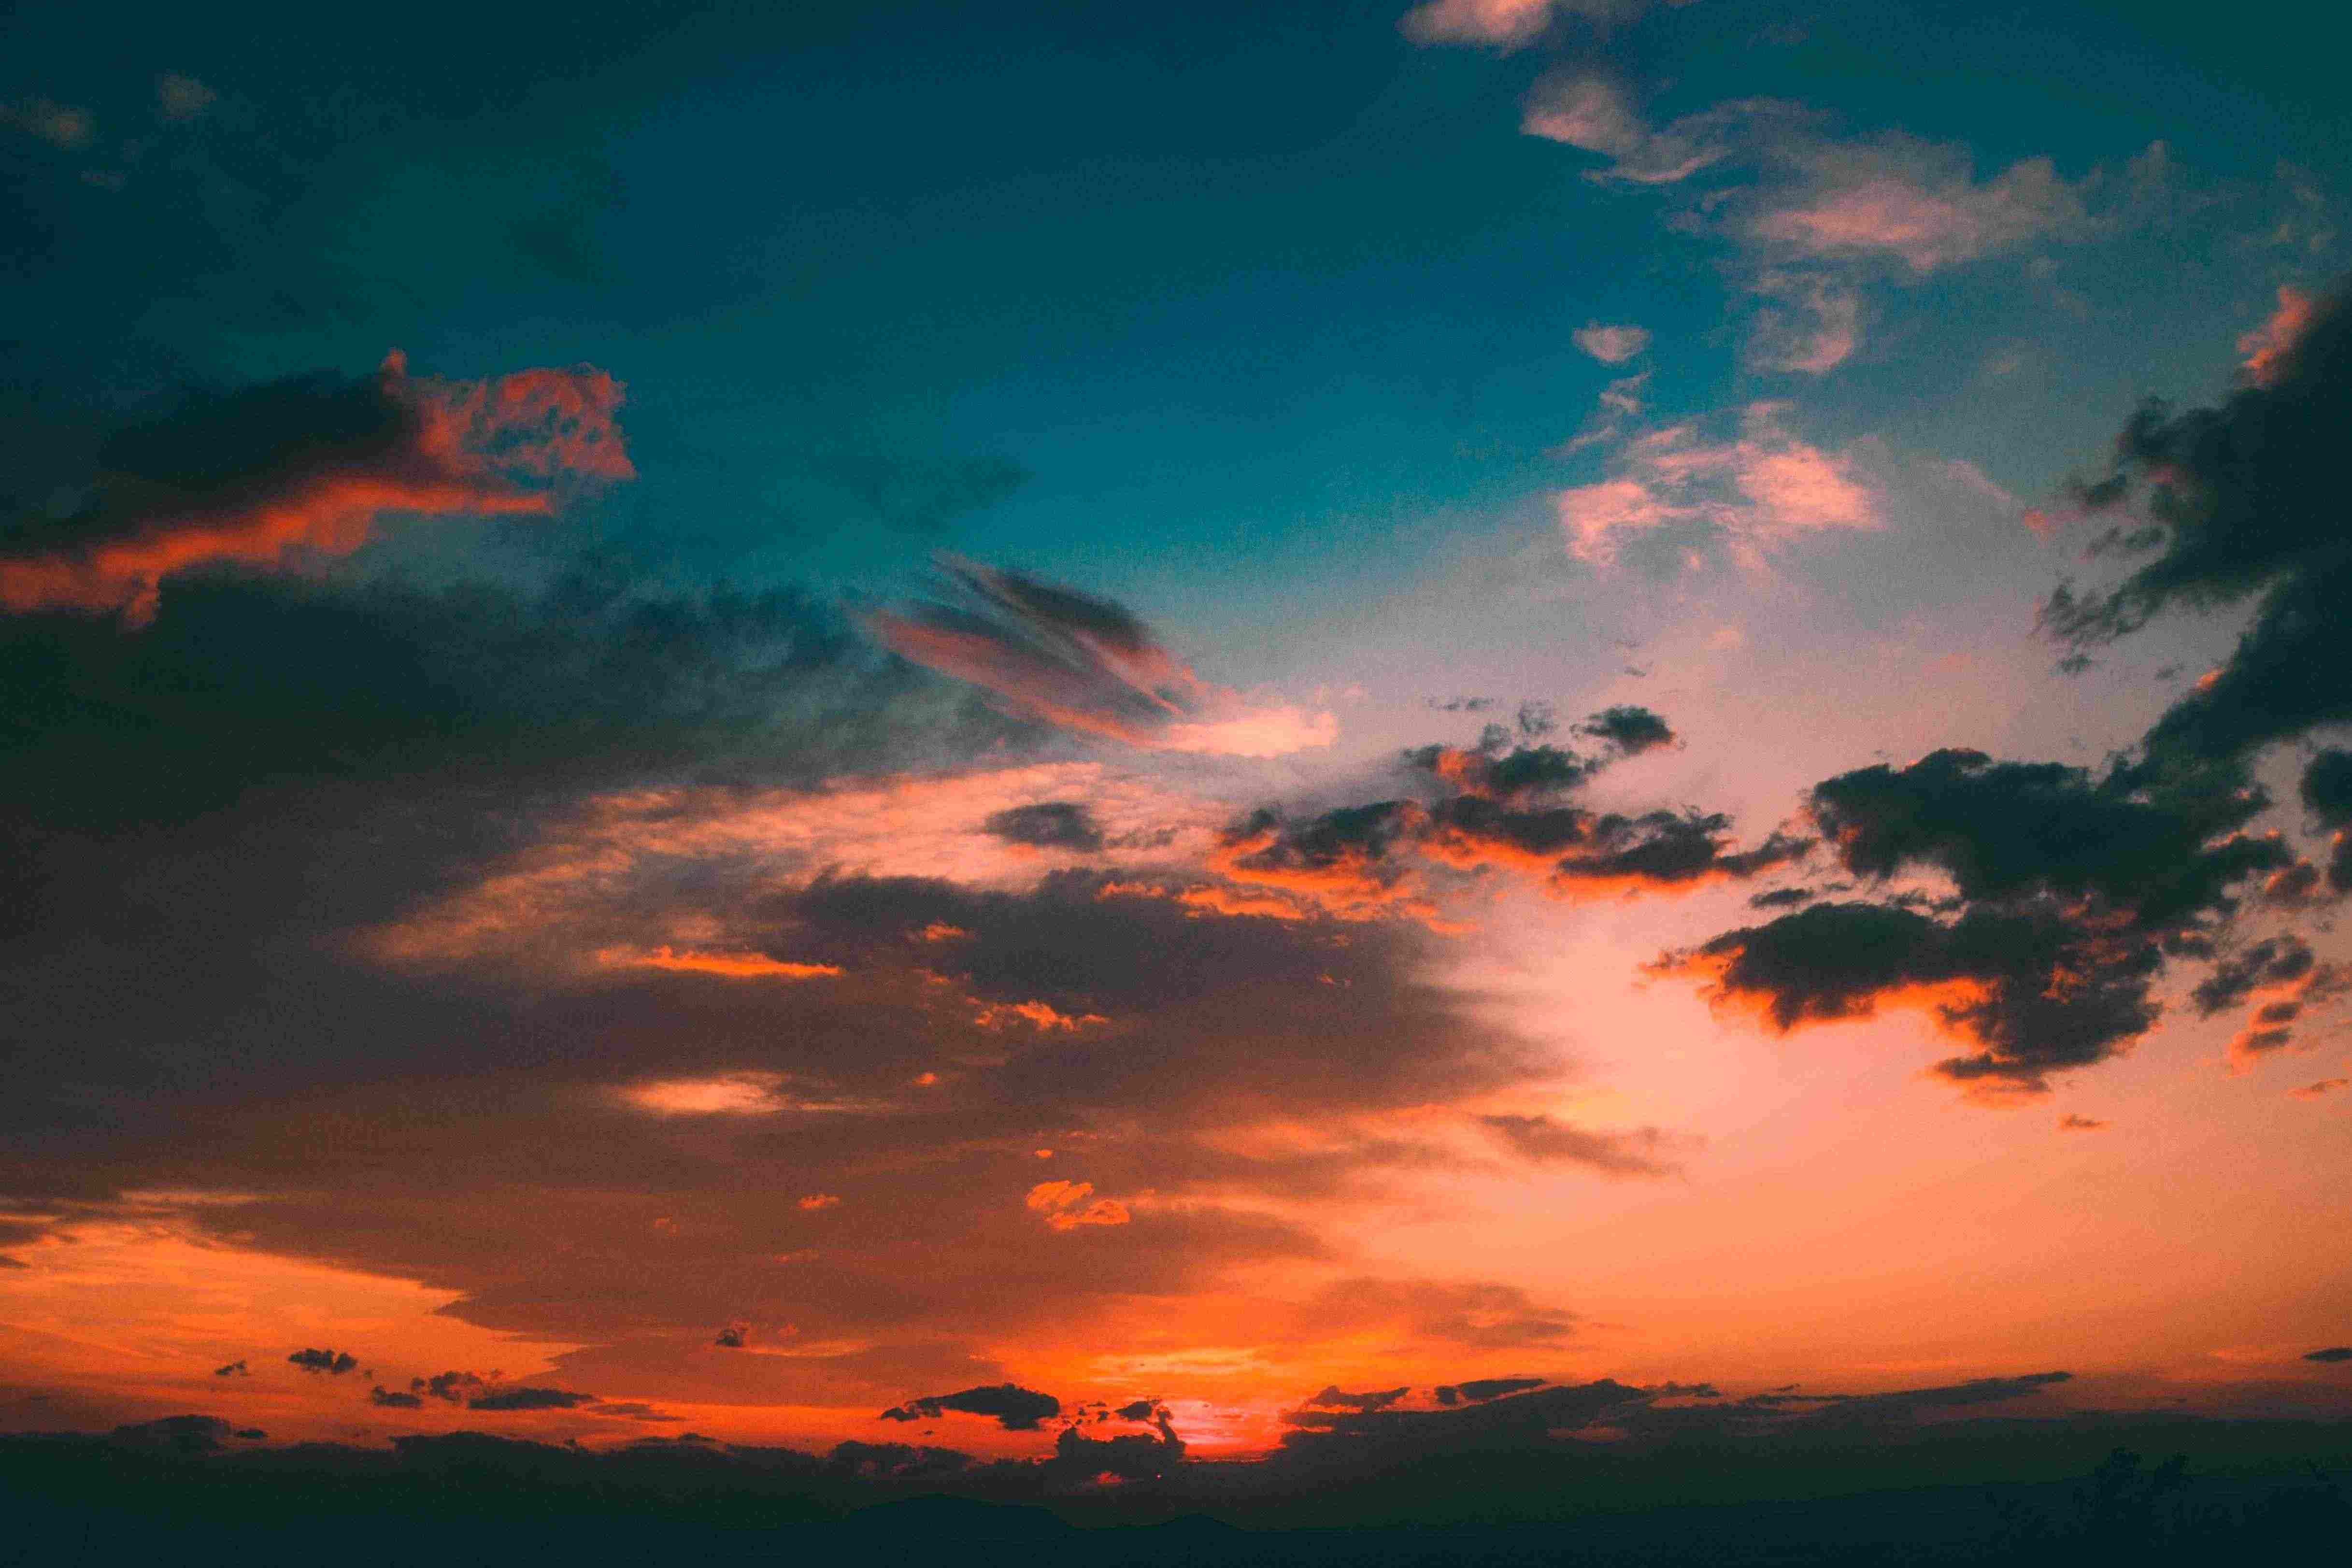
\includegraphics[width=0.8\textwidth]{sky}
    \caption{Sky}
  \end{figure}

  \blindmathtrue
  \Blinddocument
  \blindmathpaper

  \section{Table}

    \Blindtext

    \begin{table*}
      \centering
      \caption{A table extracted from
        \href{https://people.inf.ethz.ch/markusp/teaching/guides/guide-tables.pdf}
          {"Small Guide to Making Nice Tables"}}
      \begin{adjustbox}{max width=\textwidth}
        \begin{tabular}{@{}rrrrcrrrcrrr@{}}
          \toprule
          & \multicolumn{3}{c}{$w = 8$} & \phantom{abc}& \multicolumn{3}{c}{$w = 16$} &
          \phantom{abc} & \multicolumn{3}{c}{$w = 32$}\\
          \cmidrule{2-4} \cmidrule{6-8} \cmidrule{10-12}
          & $t=0$ & $t=1$ & $t=2$ && $t=0$ & $t=1$ & $t=2$ && $t=0$ & $t=1$ & $t=2$ \\
          \midrule
          $dir=1$ \\
          $c$ & 0.0790 & 0.1692 & 0.2945 && 0.3670 & 0.7187 & 3.1815 && -1.0032 & -1.7104 & -21.7969 \\
          $c$ & -0.8651& 50.0476& 5.9384&& -9.0714& 297.0923& 46.2143&& 4.3590& 34.5809& 76.9167 \\
          $c$ & 124.2756& -50.9612& -14.2721&& 128.2265& -630.5455& -381.0930&& -121.0518& -137.1210& -220.2500 \\
          $dir=0$\\
          $c$ & 0.0357& 1.2473& 0.2119&& 0.3593& -0.2755& 2.1764&& -1.2998& -3.8202& -1.2784 \\
          $c$ & -17.9048& -37.1111& 8.8591&& -30.7381& -9.5952& -3.0000&& -11.1631& -5.7108& -15.6728 \\
          $c$ & 105.5518& 232.1160& -94.7351&& 100.2497& 141.2778& -259.7326&& 52.5745& 10.1098& -140.2130 \\
          \bottomrule
        \end{tabular}
      \end{adjustbox}
    \end{table*}

  \section{Code}

  \Blindtext[5][2]

  \begin{listing}[htbp!]
    \begin{minted}[
      frame=single,
      framesep=10pt,
      fontsize=\footnotesize
    ]{python}
import numpy as np

def incmatrix(genl1,genl2):
    m = len(genl1)
    n = len(genl2)
    M = None #to become the incidence matrix
    VT = np.zeros((n*m,1), int)  #dummy variable

    #compute the bitwise xor matrix
    M1 = bitxormatrix(genl1)
    M2 = np.triu(bitxormatrix(genl2),1)

    for i in range(m-1):
        for j in range(i+1, m):
            [r,c] = np.where(M2 == M1[i,j])
            for k in range(len(r)):
                VT[(i)*n + r[k]] = 1;
                VT[(i)*n + c[k]] = 1;
                VT[(j)*n + r[k]] = 1;
                VT[(j)*n + c[k]] = 1;

                if M is None:
                    M = np.copy(VT)
                else:
                    M = np.concatenate((M, VT), 1)

                VT = np.zeros((n*m,1), int)

    return M
    \end{minted}
    \caption{Some Python code extracted from
      \href{https://www.overleaf.com/learn/latex/Code_Highlighting_with_minted}{Overleaf}
    }
  \end{listing}

  \section{Tikz diagram}

  \Blindtext

  \begin{figure}[htbp!]
    \centering
    \begin{adjustbox}{max width=\textwidth}
      \begin{tikzpicture}
        \pgfdeclarelindenmayersystem{Koch curve}{
          \rule{F -> F+F--F+F}
        }

        \draw[draw][l-system={Koch curve, step=4pt, angle=60, axiom=F++, order=5}]
        lindenmayer system;
      \end{tikzpicture}
    \end{adjustbox}
    \caption{Koch curve~\cite{koch}}
  \end{figure}


  \begin{listing}[htpb!]
    \begin{minted}[
      frame=single,
      framesep=10pt,
      fontsize=\footnotesize
    ]{yaml}
axiom: F++
rules:
  F => F+F--F+F
angle: 60
order: 5
    \end{minted}
    \caption{Koch curve can be produced using a Lindenmayer system}
  \end{listing}

  \blindtext

  \begin{figure}[htbp!]
    \centering
    \tiny  
    \pipar{3 . 1 4 1 5 9 2 6 5 3 5 8 9 7 9 3 2 3 8 4 6 2 6 4 3 3 8 3 2 7 9 5 0 2 8 8 4 1 9 7 1 6 9 3 9 9 3 7 5 1 0 5 8 2 0 9 7 4 9 4 4 5 9 2 3 0 7 8 1 6 4 0 6 2 8 6  2 0 8 9 9 8 6 2 8 0 3 4 8 2 5 3 4 2 1 1 7 0 6 7 9 8 2 1 4 8 0 8 6 5 1 3 2 8 2 3 0 6 6 4 7 0 9 3 8 4 4 6 0 9 5 5 0 5 8 2 2 3 1 7 2 5 3 5 9 4 0 8 1 2 8 4 8 1  1 1 7 4 5 0 2 8 4 1 0 2 7 0 1 9 3 8 5 2 1 1 0 5 5 5 9 6 4 4 6 2 2 9 4 8 9 5 4 9 3 0 3 8 1 9 6 4 4 2 8 8 1 0 9 7 5 6 6 5 9 3 3 4 4 6 1 2 8 4 7 5 6 4 8 2 3 3  7 8 6 7 8 3 1 6 5 2 7 1 2 0 1 9 0 9 1 4 5 6 4 8 5 6 6 9 2 3 4 6 0 3 4 8 6 1 0 4 5 4 3 2 6 6 4 8 2 1 3 3 9 3 6 0 7 2 6 0 2 4 9 1 4 1 2 7 3 7 2 4 5 8 7 0 0 6  6 0 6 3 1 5 5 8 8 1 7 4 8 8 1 5 2 0 9 2 0 9 6 2 8 2 9 2 5 4 0 9 1 7 1 5 3 6 4 3 6 7 8 9 2 5 9 0 3 6 0 0 1 1 3 3 0 5 3 0 5 4 8 8 2 0 4 6 6 5 2 1 3 8 4 1 4 6  9 5 1 9 4 1 5 1 1 6 0 9 4 3 3 0 5 7 2 7 0 3 6 5 7 5 9 5 9 1 9 5 3 0 9 2 1 8 6 1 1 7 3 8 1 9 3 2 6 1 1 7 9 3 1 0 5 1 1 8 5 4 8 0 7 4 4 6 2 3 7 9 9 6 2 7 4 9  5 6 7 3 5 1 8 8 5 7 5 2 7 2 4 8 9 1 2 2 7 9 3 8 1 8 3 0 1 1 9 4 9 1}
    \caption{The shape of $\pi$ with the digits of $\pi$. Source: \href{https://tex.stackexchange.com/a/160438}{\TeX{} Stack Exchange}}
  \end{figure}


\blindtext

  \bibliographystyle{unsrt}
  \bibliography{bibliography}
\end{document}
